\begin{center}
    \section{Приложение B}\label{appendix:B}
    \textbf{\Large{Спин. Математический и физический подход}}
\end{center}

План:
\begin{enumerate}
    \item Опыт Штерна -- Герлаха. Сфера Блоха.
    \item Матрицы для вращения поляризации. SO(3), SU(2) матрицы. Сравнение со спинами.
    \item Матрицы и вектора паули. Вращение спиноров.
    \item Сравнение с квантернионами. Группы и алгебра Клиффорда.
\end{enumerate}

Рассказывать про спин в приложении -- затея крайне непростая, так как его строгое математическое описание требует как минимум страниц 30 и пары-тройки семинаров. В связи с этим, я постараюсь дать базовое описание математики спиноров и физики спина. В конце я оставлю ссылки на источники, используя которые я разбирался в этой достаточно запутанной теме. Если вас заинтересует более глубокое понимание -- обязательно пройдите по ссылкам, посмотрите видео и почитайте книги или статьи по этой теме. 

Говорить мы будем в основном не про сам спин, а про объект, которым его описывают математический -  \textit{спинор}. Однако, я попытаюсь не уходить от основной темы и в случае чего всегда возвращаться к ``физике'' процесса. На этом лирические отступления закончены, давайте преступим к изучению спинов и спиноров.

\subsection{Опыт Штерна -- Герлаха}
\hspace{1em} Наверняка подкованный читатель уже много раз слышал про этот эксперимент, однако для полноты картины я не могу обойти его стороной. Поэтому, если вы уверены, что хорошо понимаете суть опыта и вам не нужно напоминать про причину возникновения такого понятия как спин -- можете спокойно пропустить этот параграф и пойти к следующему.

Опыт состоит в пропускании пучка нейтральных частиц (например, атомов серебра) через неоднородное магнитное поле. Схему установки можно посмотреть на рисунке \ref{fig B.1}. Во время проведения эксперимента главенствовала Боровская модель атома, представляющая собой ядро и крутящиеся вокруг него электроны. Исходя из этой модели, в нейтральных атомах магнитное поле, образованное орбитальным моментом, должно распределяться равномерно, образуя на экране прямую линию. На деле же оказалось, что после вылета из магнита частицы летели только в двух направлениях. Это повлекло за собой следующий вывод -- у частиц есть ``внутренний'' магнитный момент, который ещё и квантуется. Его назвали \textit{спин}, так как сначала было предположение, что электрон крутится вокруг своей оси. В итоге оказалось, что это предположение ошибочное и модель Бора в целом неверна, хотя и даёт правильный вектора понимания устройства атома.
\begin{figure}[h!]
\centering
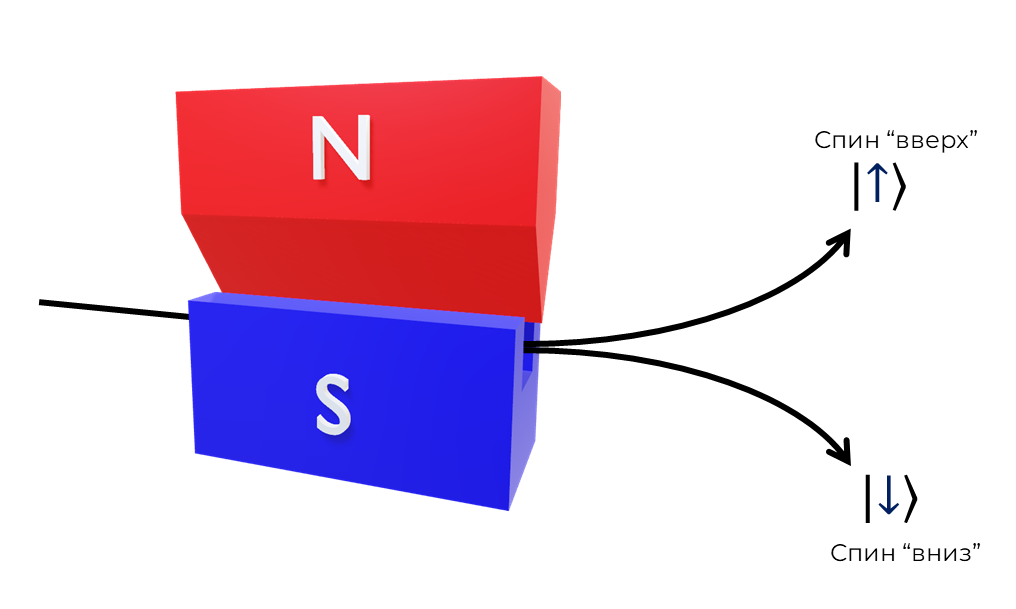
\includegraphics[scale=0.4]{appendix/images/gc.png}
\caption{Магнит с неоднородным магнитным полем. Частицы после вылета попадали на экран.}
\label{fig B.1}
\end{figure}

Итак, у нас есть два состояния - частица летит вверх и частица летит вниз. Пусть вертикальная ось будет ось Z. Обозначим тогда состояние частицы, спин которой направлен "вверх" как $\ket{z}$. Тогда, для частицы со спином вниз будет $\ket{-z}$. Так как частица в момент измерения (т.е. в момент попадания на экран) может оказаться только в одном из состояний, мы считаем, что эти состояния ортогональны. Тогда, если добавить в установку \ref{fig B.1} ещё один магнит, на пути верхней траектории, то частица после второго магнита полетит наверх с вероятностью 1. В формализме квантовой механике это можно записать как:
\[
|\bra{z}\ket{z}|^2 = |\bra{-z}\ket{-z}|^2 = 1,\; |\bra{-z}\ket{z}|^2 = 0
\]
Если мы положим магнит на бок так, что магнитное поле будет направлено вдоль оси X, тогда у нас получится аналогичный результат для состояний $\ket{x}$ и $\ket{-x}$:
\[
|\bra{x}\ket{x}|^2 = |\bra{-x}\ket{-x}|^2 = 1,\;|\bra{-x}\ket{x}|^2 = 0
\]

Разнообразим картину -- пусть подряд идут два магнита, но с разными направлениями. Поставим на пути части, пролетевших первый магнит с состоянием $\ket{z}$, магнит, измеряющий состояние по оси X. Оказывается, вероятность пролететь в ``положительном'' или ``отрицательном'' направлении будет одинаковая и равна 1/2. Другими словами:
\[
|\bra{x}\ket{z}|^2 = |\bra{-x}\ket{z}|^2 = 1/2
\]
Как известно, состояние в квантовой механике можно представить в виде линейной комбинации ``базисных'' состояний. Тогда, разложим состояние $\ket{x}$ как:
\[
\ket{x} = \alpha\ket{z} + \beta\ket{-z}
\]
Из полученной выше вероятности легко найти коэффициенты перед $z$ состояниями:
\[
\ket{x} = \frac{1}{\sqrt{2}}\ket{z} + \frac{1}{\sqrt{2}}\ket{-z}
\]
Из условия ортогональности, получим коэффициенты для состояния $\ket{-x}$:
\[
\ket{-x} = \frac{1}{\sqrt{2}}\ket{z} - \frac{1}{\sqrt{2}}\ket{z}
\]

Для направления по оси Y распределение вероятностей будет точно такое же, как и для оси X. Но те же самые коэффициенты мы взять не можем. Поэтому, чтобы описать состояние $\ket{y}$, будем использовать комплексные числа:
\begin{gather*}
\ket{y} = \frac{1}{\sqrt{2}}\ket{z} + \frac{i}{\sqrt{2}}\ket{-z}\\
\ket{-y} = \frac{1}{\sqrt{2}}\ket{z} - \frac{i}{\sqrt{2}}\ket{-z}
\end{gather*}
Домножение на комплексный множитель не изменяет состояние при измерении, так как берётся квадрат модуля. Поэтому, результаты при подсчёте будут точно такие же.

Обратим внимание на следующий важный момент. Физически состояния $z$ и $-z$ являются антипараллельными, так как частица летит либо вверх, либо вниз. В свою очередь состояния $x$ и $-x$ ортогональный им (рисунок \ref{fig B.2b}). В это же время, соответствующие квантовые состояния имеют следующие отношения: $\ket{z}$ и $\ket{-z}$ ортогональный, а между $\ket{x}$ и $\ket{z}$ угол составляет 45 градусов (рисунок \ref{fig B.2a}). Таким образом, отношение углов между квантовыми состояниями и физическими состояниями соотносится как 1:2. Получается, для полного поворота на 360 градусов в пространстве квантовых состояний необходимо два полных поворота на 720 в физическом пространстве. Это проявление одного из свойств спиноров, о которых мы поговорим далее.

\begin{figure}[!h]
  \centering
  \subfloat[Пространство квантовых состояний]{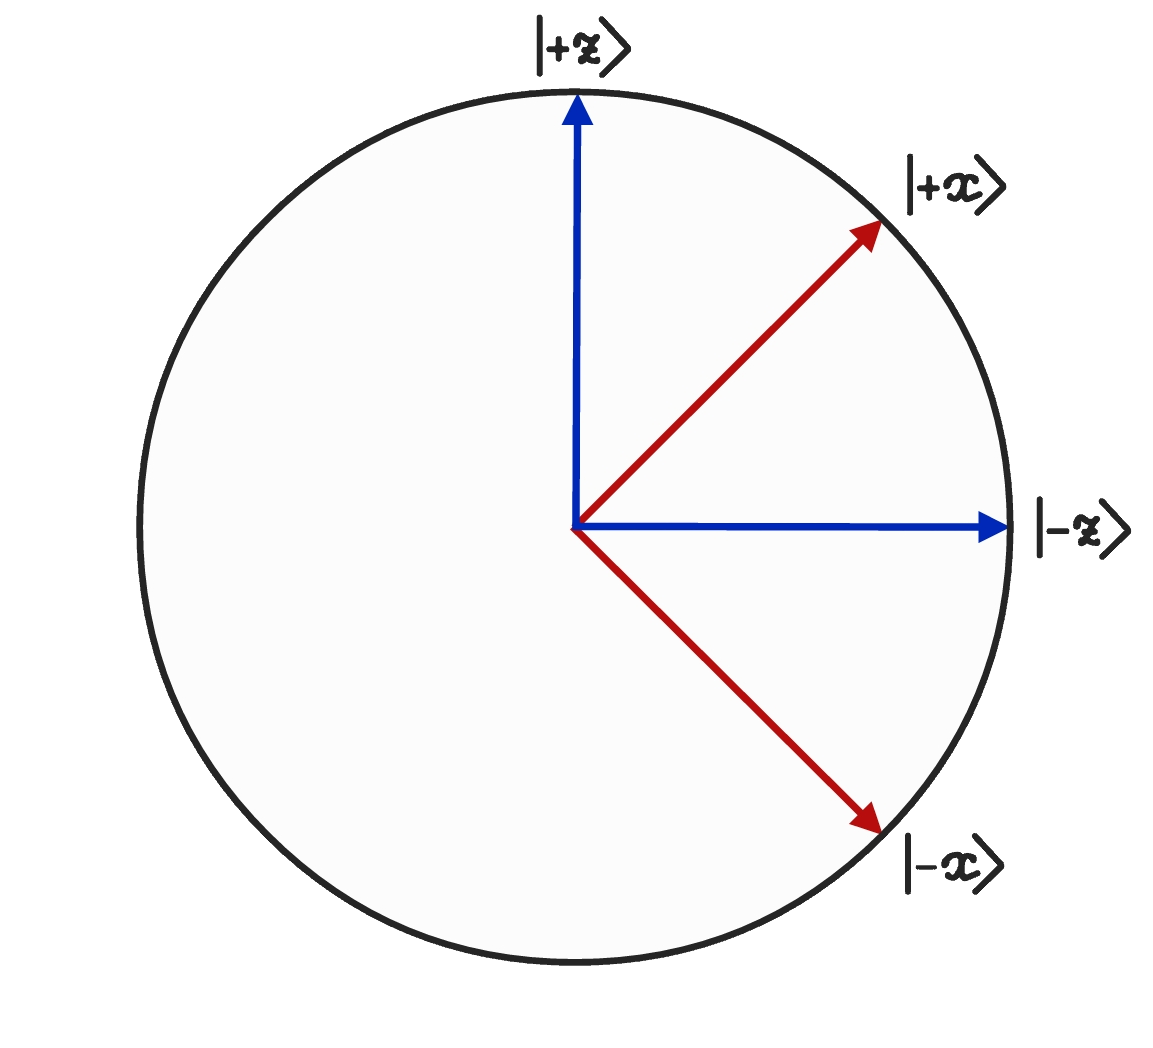
\includegraphics[scale=0.24]{appendix/images/qspace.png}\label{fig B.2a}}
  \hfill
  \subfloat[Физическое пространство]{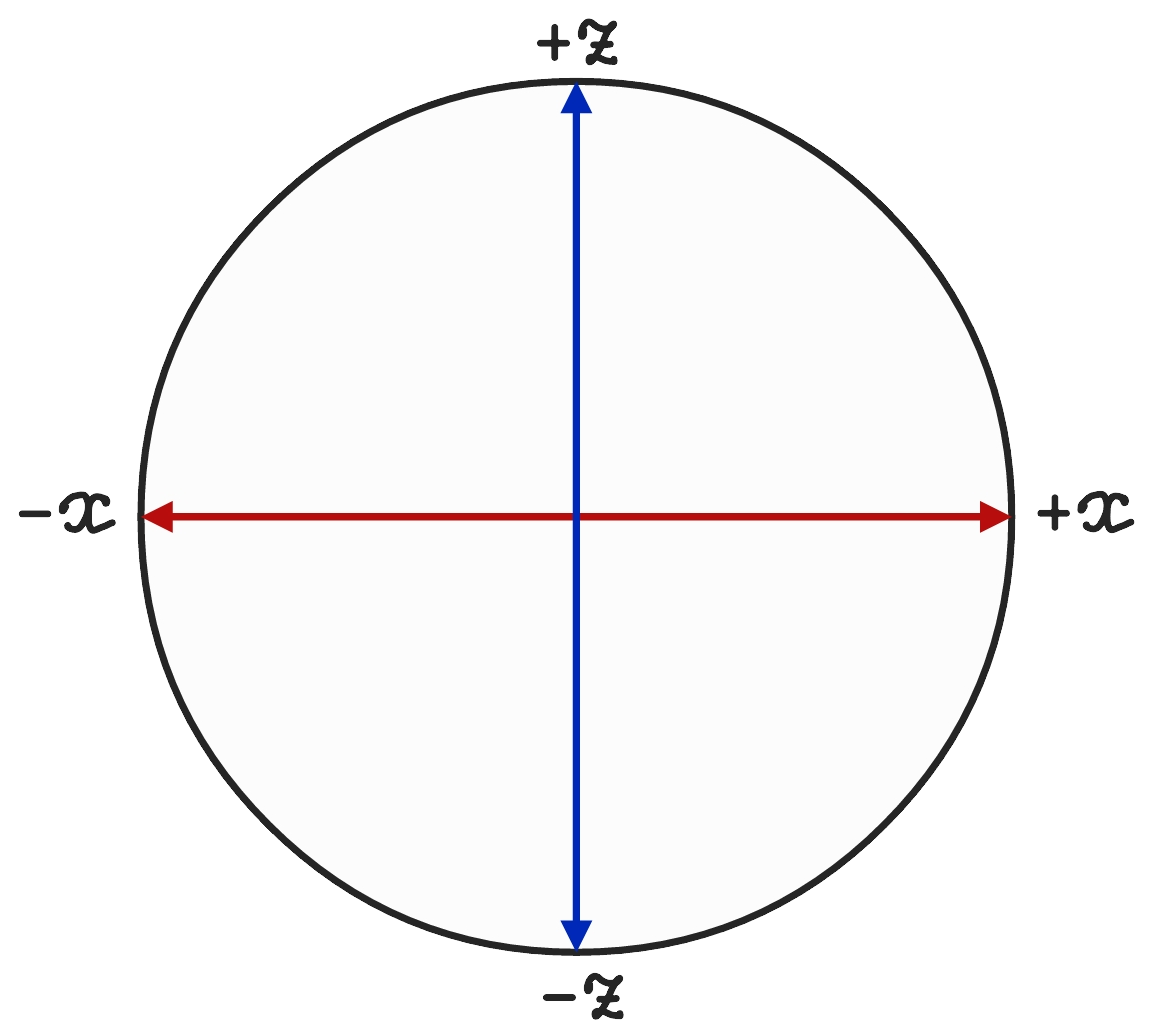
\includegraphics[scale=0.24]{appendix/images/physical space.png} \label{fig B.2b}}
  \caption{}
\end{figure}

В физическом пространстве для представления двухуровневых квантовых состояний используется сфера блоха (рисунок \ref{fig B.3}). Так, состояние $\ket{z}$ можно представить как вектор, направленный вдоль положительной оси Z. Для того, чтобы разобраться, как описывать состояния со спином 1/2 и разобраться со спинорами, нужно обсудить, каким образом вращаются и перемещаются по сфере квантовые состояния. Этим мы и будем заниматься в следующих параграфах.
\begin{figure}[h!]
\centering
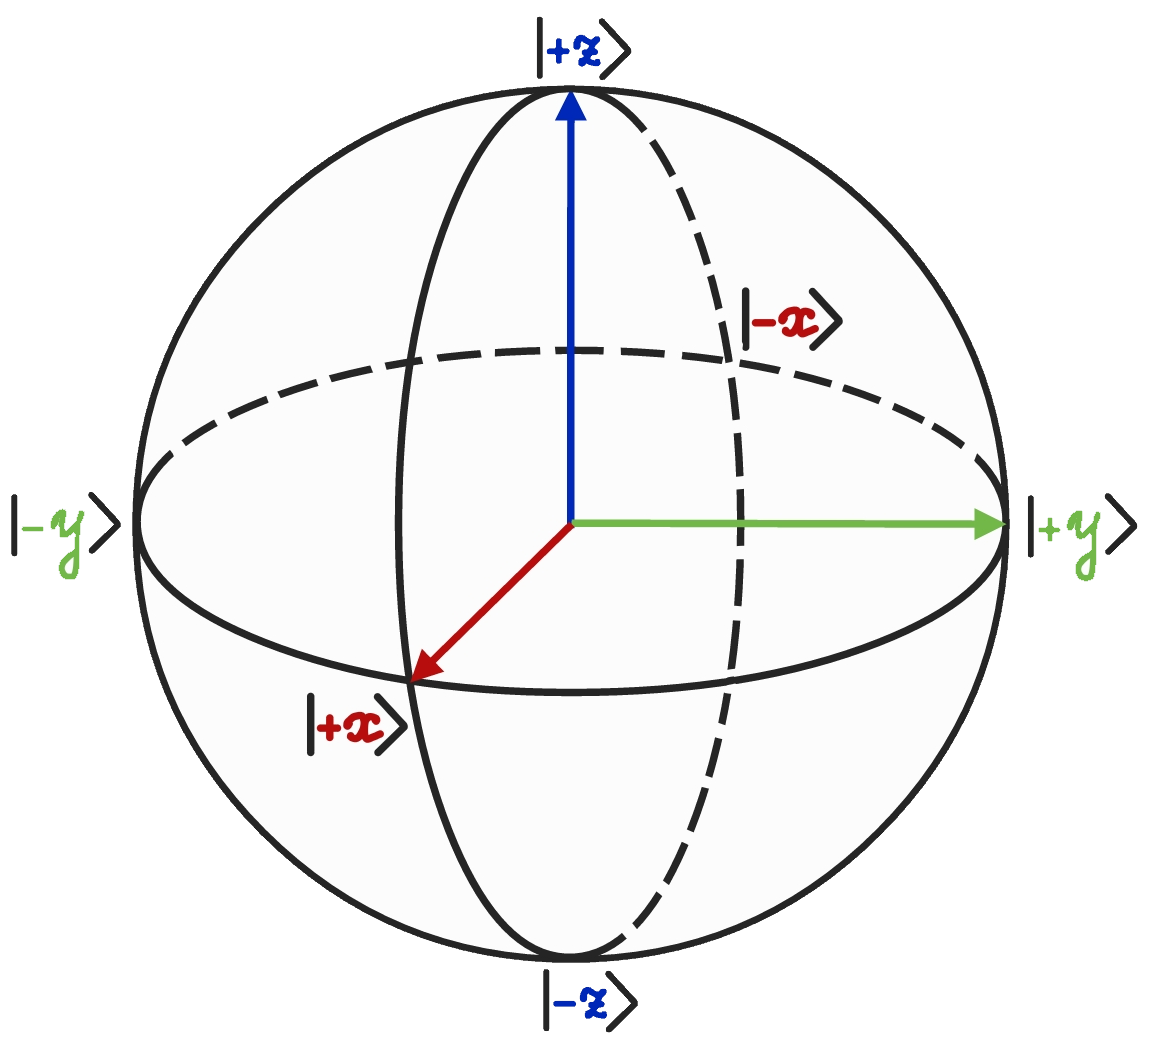
\includegraphics[scale=0.23]{appendix/images/bloch sphere.png}
\caption{Сфера блоха}
\label{fig B.3}
\end{figure}

\subsection{Поляризация света}
Сделаем небольшое отступление от квантовой механики в сторону оптики для того, чтобы укрепить связь между реальной физикой и объектами, используемыми для описания поворота в пространстве. Тем более, с курсом оптики вы уже знакомы, так что многое здесь для вас будет известным и понятным.
\subsubsection{Векторы Джонса}
Поляризацией света можно назвать направление вектора электрического или магнитного поля во время его распространения (рисунок \ref{fig B.4}). Далее в параграфе будем рассматривать только вектор, связанные с электрическим полем. Разложим его в линейную комбинацию трёх базисных векторов:
\[
\Vec{E} = E_x \Vec{e}_x + E_y \Vec{e}_y + E_z \Vec{e}_z
\]
Рассмотрим вертикальную поляризацию. В этом случае $E_z = E_x = 0$. Распишем компоненту $E_y$ :
\[
E_y = A_y \cos(\omega t - kz + \phi_y)
\]
или, используя экспоненциальную форму
\[
E_y = A_y e^{i\phi_y}e^{\omega t - kz}.
\]
Замечу, что если во второй формуле взять реальную часть, получим первую. Так как у нас поляризация реально физическое явление, то в эксперименте мы рассматриваем как раз реальную часть, поэтому такой переход более чем законен.
\begin{figure}[h!]
\centering
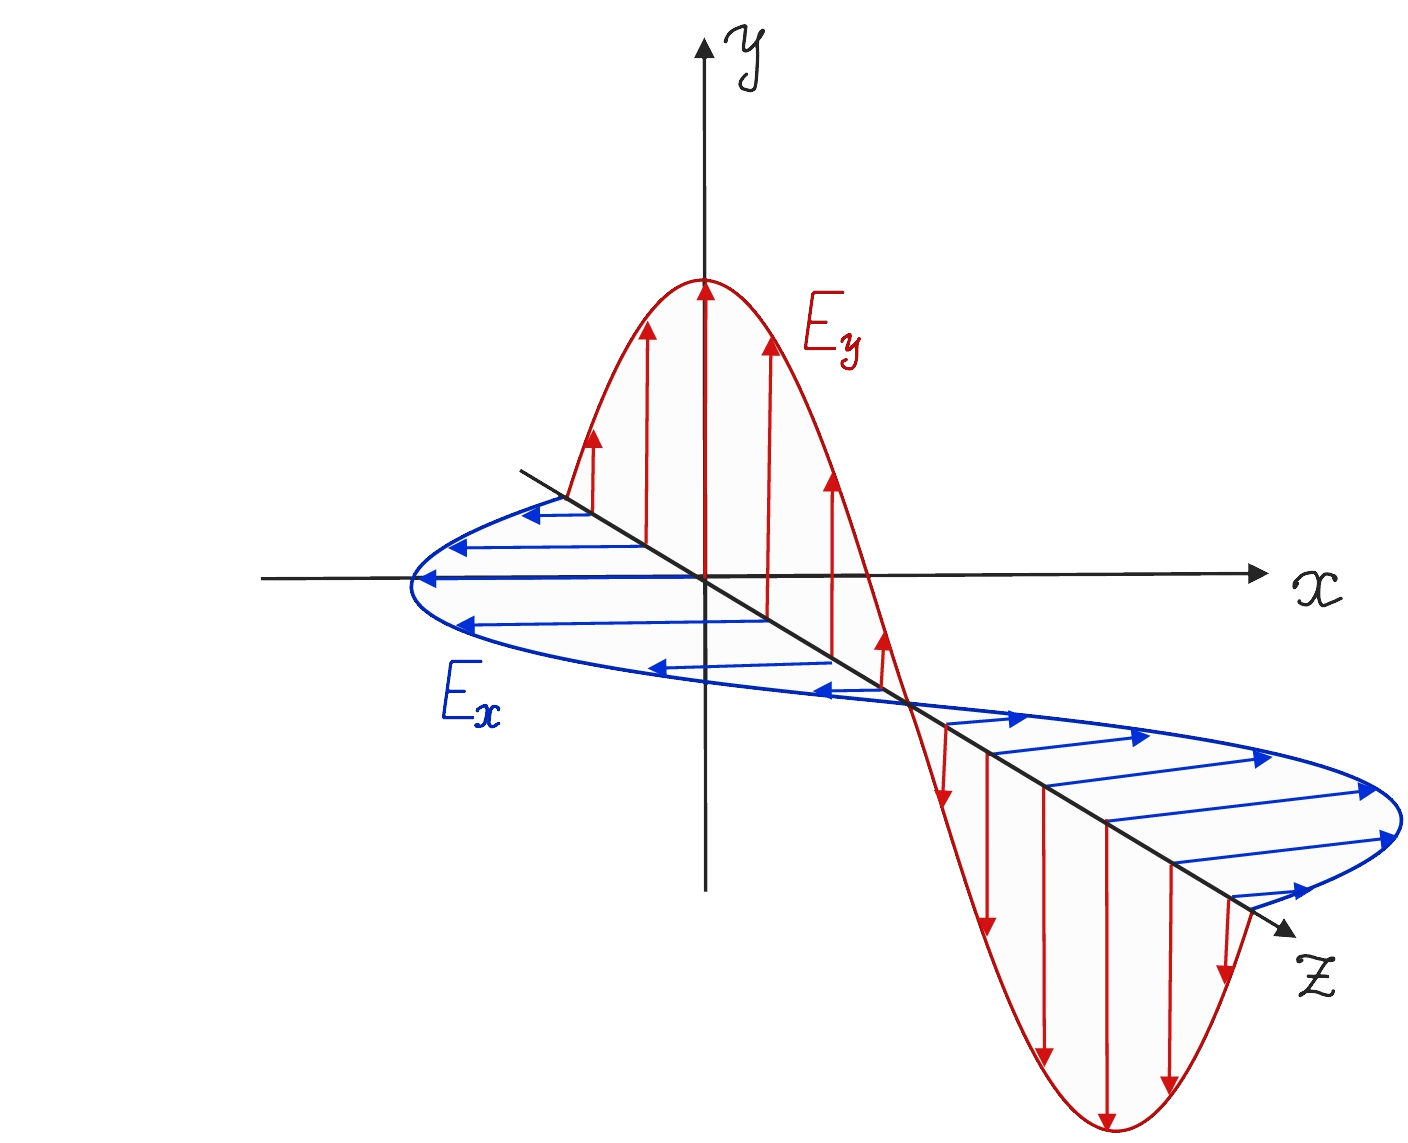
\includegraphics[scale=0.23]{appendix/images/polarization.png}
\caption{Распространение волны вдоль оси Z}
\label{fig B.4}
\end{figure}

Для горизонтальной компоненты аналогично:
\[
E_x = A_x e^{i\phi_x}e^{\omega t - kz}.
\]
Компонента $E_z$ в нашем случае определяет то, в какую сторону будет двигаться волна. Поэтому, мы всегда можем определить координаты так, чтобы эта компонента была равна 0. Тогда, вектор $\Vec{E}$ можно записать в виде
\[
\begin{bmatrix} E_x\\ E_y\\ 0 \end{bmatrix} = \begin{bmatrix} A_x e^{i\phi_x}e^{\omega t - kz}\\ A_y e^{i\phi_y}e^{\omega t - kz}\\ 0 \end{bmatrix}
\]
Легко заметить, что для полного описания поляризации волны нам достаточно знать фазу $\phi$ и амплитуду $A$, так как множитель $e^{\omega t - kz}$ одинаковы для всех членов. Помимо этого, мы можем выкинуть из вектора третий член -- при правильном выборе координат он всегда будет равен 0. Таким образом, мы приходим к \textit{векторам Джонса} -- векторам с двумя членами, описывающими поляризацию волны.
\[
\begin{bmatrix} A_x e^{i\phi_x}e^{\omega t - kz}.\\ A_y e^{i\phi_y}e^{\omega t - kz}\\ 0 \end{bmatrix} \rightarrow \Vec{J} = \begin{bmatrix} A_x e^{i\phi_x}\\ A_y e^{i\phi_y}\end{bmatrix}
\]

Вектор Джонса можно записать в виде линейной комбинации вертикальной и горизонтальной поляризации:
\[
\Vec{J} = A_x e^{i\phi_x}\begin{bmatrix} 1 \\ 0 \end{bmatrix} + A_y e^{i\phi_y}\begin{bmatrix} 0 \\ 1 \end{bmatrix} = A_x e^{i\phi_x}\Vec{H} + A_y e^{i\phi_y}\Vec{V}
\]
Теперь найдём, как используя вектор Джонса описать известные нам диагональную и левую круговую поляризацию. Пусть в обоих членах амплитуда будет равна 1, а фаза равна 0. Тогда, получим сумму двух перпендикулярных векторов с длинной 1. Из прямоугольного треугольника, построенного на этих векторах, находим, что длинна их суммы равна $\sqrt{2}$. Значит, чтобы суммарный вектор получился нормированным, необходимо оба члена разделить на $\frac{1}{\sqrt{2}}$. Назовём его $\Vec{D}$ и запишем его разложение:
\[
\Vec{D} = \frac{1}{\sqrt{2}}\Vec{H} + \frac{1}{\sqrt{2}}\Vec{V}
\]
Ничего не напоминает? Не будем сильно спешить, но я думаю внимательный читатель уже заметил сходство с разложением состояния $\ket{x}$ по базисным состояниям $\ket{z}$ и $\ket{-z}$. Точно также мы можем представить антидиагональную поляризацию $\Vec{A}$, поменяв сумму векторов на разность:
\[
\Vec{A} = \frac{1}{\sqrt{2}}\Vec{H} - \frac{1}{\sqrt{2}}\Vec{V}
\]
Расположение векторов Джонса можно посмотреть на рисунке \ref{fig B.5}
\begin{figure}[h!]
\centering
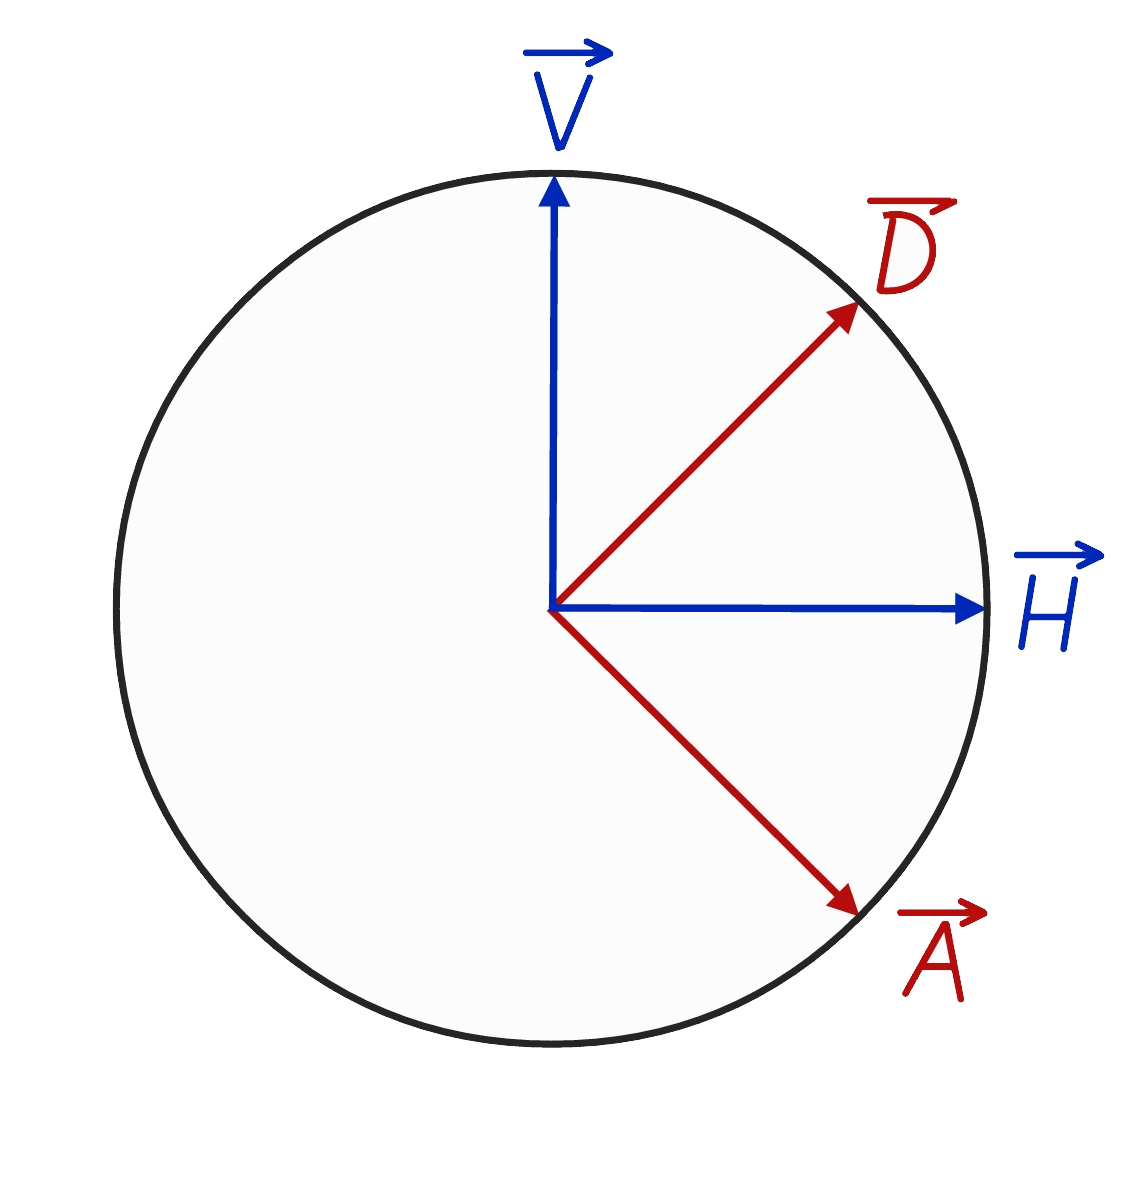
\includegraphics[scale=0.23]{appendix/images/pol phys space.png}
\caption{Расположение векторов Джонса}
\label{fig B.5}
\end{figure}

Рассмотрим ещё одну, более сложную поляризацию. Пусть амплитуда так же равна единице, однако фаза при вертикальной поляризации равна $\pi/2$, то есть:
\[
\Vec{J} = \Vec{H} + e^{i\frac{\pi}{2}}\Vec{V}
\]
Для анализа выберем частоту $\omega = 1$ и $z = 0$. Тогда, вспоминая про наш дополнительный член, который мы вынесли за вектор, можем сделать следующую цепочку преобразований:
\begin{align*}
(\begin{bmatrix} 1 \\ 0 \end{bmatrix} + \begin{bmatrix} 0 \\ e^{i\frac{\pi}{2}} \end{bmatrix})e^{it} = \begin{bmatrix} 1 \\ e^{i\frac{\pi}{2}} \end{bmatrix} e^{it} = \begin{bmatrix} e^{it} \\ e^{i(\frac{\pi}{2} + t)} \end{bmatrix} \rightarrow \begin{bmatrix} \cos t \\ \cos(\frac{\pi}{2} + t) \end{bmatrix} = \begin{bmatrix} \cos t \\ -\sin t \end{bmatrix}
\end{align*}
Подставляя разные значения t, можно заметить, что поляризация вращается по часовой стрелке. Действительно, при $t = 0$ вектор Джонса будет равен $\Vec{H}$, при $t = \frac{\pi}{2}$ вектор равен $-\Vec{V}$ и так далее. Этот вектор будем называть левой круговой поляризацией и обозначать $\Vec{L}$. Ортогональный ему, вектор правой круговой поляризации будем обозначать $\Vec{R}$. Запишем их разложение через вектор $\Vec{H}$ и вектор $\Vec{V}$ сразу с нормировкой:
\begin{gather*}
    \Vec{L} = \frac{1}{\sqrt{2}}\Vec{H} + \frac{i}{\sqrt{2}}\Vec{V}\\
    \Vec{R} = \frac{1}{\sqrt{2}}\Vec{H} - \frac{i}{\sqrt{2}}\Vec{V}
\end{gather*}
Здесь, по формуле Эйлера мы заменили $e^{i\pi/2}$ на $i$.

Итак, как и в случае со спинами, мы нашли 6 состояний, которые описывают любую возможную поляризацию. На самом деле, вектора Джонса ведут себя точно так же, как и спиноры, поэтому являются отличной иллюстрацией последних. В физическом пространстве найденные вектора Джонса между собой ортогональный. Давайте покажем, что в ``поляризационном'' пространстве угол между векторами будет в два раза больше. Для этого посмотрим, как осуществляется переход от одного состояния к другому.
\subsubsection{Матрицы Джонса. Сфера Пуанкаре}
Для вращений векторов Джонса мы используем, как это не удивительно, матрицы Джонса. У них тоже есть физическое воплощение -- волновые пластины. Так, четвертьволновой пластине, которая меняет фазу на $\pi/2$, соответствует матрица $\begin{bmatrix} 1 & 0 \\ 0 & i \end{bmatrix}$. Давайте посмотрим, как она будет действовать на диагональную поляризацию:
\[
\begin{bmatrix} 1 & 0 \\ 0 & i \end{bmatrix}\Vec{D} = \frac{1}{\sqrt{2}}\begin{bmatrix} 1 & 0 \\ 0 & i \end{bmatrix}\begin{bmatrix} 1 \\ 1 \end{bmatrix} = \frac{1}{\sqrt{2}}\begin{bmatrix} 1 \\ i \end{bmatrix} = \Vec{L}
\]
Значит, диагональная поляризация под действием четвертьволновой пластинки переходит в левую круговую поляризацию. Если поставить ещё несколько пластинок, то цепочка переходов будет следующая: $\Vec{D} \rightarrow \Vec{L} \rightarrow \Vec{A} \rightarrow \Vec{R}\rightarrow \Vec{D}$.

Если попробовать подействовать пластинкой на горизонтальную поляризацию, то легко убедиться, что ничего не поменяется. Однако, можно провести трюк -- если повернуть пластину на $45^{\circ}$, то поляризация для неё станет диагональной. С математической точки зрения нам нужно повернуть сначала повернуть базис на $\pi/4$, затем подействовать пластинкой, затем повернуть базис обратно. Запишем матрицу, которая получится при последовательном выполнении этих действий:
\[
\begin{bmatrix} \cos \frac{\pi}{4} & \sin \frac{\pi}{4} \\ -\sin \frac{\pi}{4} & \cos \frac{\pi}{4} \end{bmatrix} \begin{bmatrix} 1 & 0 \\ 0 & i \end{bmatrix} \begin{bmatrix} \cos \frac{\pi}{4} & -\sin \frac{\pi}{4} \\ \sin \frac{\pi}{4} & \cos \frac{\pi}{4} \end{bmatrix} = \frac{1}{2} \begin{bmatrix} 1 + i& -1 + i \\ -1 + i & 1 + i \end{bmatrix} = \frac{1}{\sqrt{2}}\begin{bmatrix} 1 & i \\ i & 1 \end{bmatrix}e^{i\frac{\pi}{4}}
\]
Попробуем применить это преобразование к вектору Джонса $\Vec{H}$, описывающему горизонтальную поляризацию:
\[
e^{i\frac{\pi}{4}}\frac{1}{\sqrt{2}}\begin{bmatrix} 1 & i \\ i & 1 \end{bmatrix}\begin{bmatrix} 1  \\ 0 \end{bmatrix} = e^{i\frac{\pi}{4}}\frac{1}{\sqrt{2}}\begin{bmatrix} 1  \\ i \end{bmatrix} = e^{i\frac{\pi}{4}}\Vec{L}
\]
Результат более чем ожидаемый. Далее я буду опускать фазовый множитель, так как он не влияет на поляризацию. Действительно, домножение элементов вектора Джонса на комплексное значение даст просто смещение волны относительно оси z, однако поляризация останется та же. Осталось определить матрицу для перехода от поляризации $\Vec{H}$ к поляризации $\Vec{A}$:
\[
\frac{1}{\sqrt{2}}\begin{bmatrix} 1 & 1 \\ -1 & 1 \end{bmatrix}\begin{bmatrix} 1  \\ 0 \end{bmatrix} = \frac{1}{\sqrt{2}}\begin{bmatrix} 1  \\ -1 \end{bmatrix}
\]
Теперь у нас есть три матрицы, используя которые мы можем переходить к любой из найденных нами 6 поляризаций. Смотря на цепочки преобразований, можно составить сферу Пуанкаре (рисунок \ref{fig B.6}). По ней видно, что, в отличие от физического пространства, ортогональные поляризации (например $\Vec{H}$ и $\Vec{V}$) находятся под углом $180^{\circ}$ друг к другу. То есть ситуация аналогична ситуации со спинами.
\begin{figure}[h!]
\centering
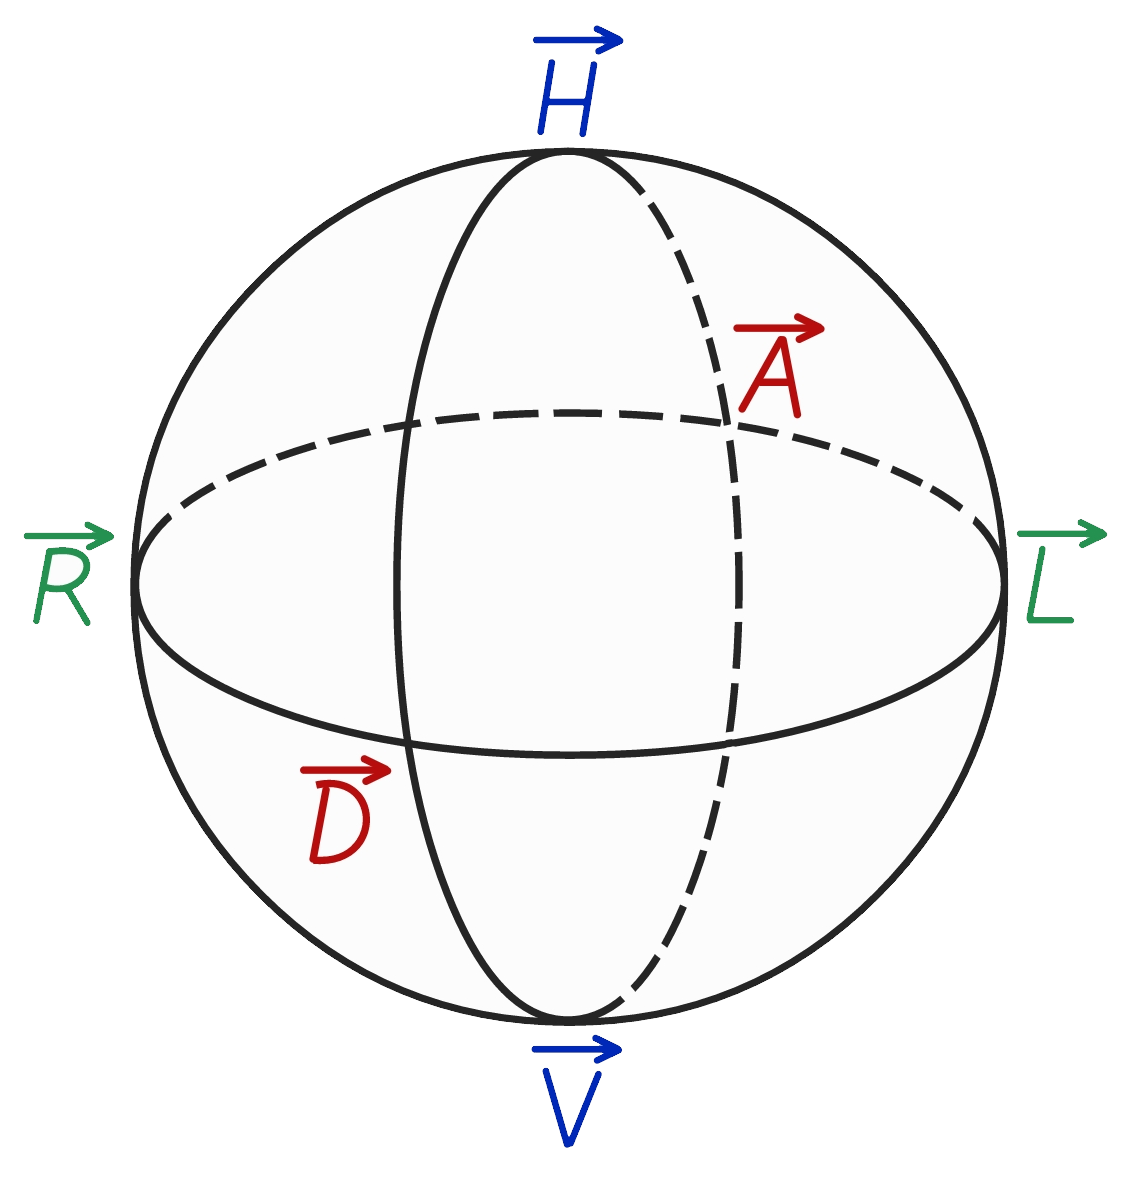
\includegraphics[scale=0.23]{appendix/images/Poincare sphere.png}
\caption{Сфера Пуанкаре}
\label{fig B.6}
\end{figure}

\subsection{Группа вращений SO(3) и SU(2), их связь}
Теперь, когда мы рассмотрели физические примеры спиноров, давайте поговорим про то, каким образом описывается их поворот в пространстве. Для этого вспомним линейную алгебру и разберёмся с ортогональными и унитарными преобразованиями.

Итак, мы хотим поворачивать вектор в трёхмерном пространстве, не изменяя его длины. Так как длина вектора определяется как квадрат нормы, нам необходимо, чтобы выполнялось следующее условие:
\[
\Vec{v} \rightarrow R\Vec{v}, \; ||\Vec{v}||^2 = ||R\Vec{v}||^2
\]
Тогда, записав норму как $v^Tv$, получим ограничение на матрицу $R$:
\[
||\Vec{v}||^2 = \Vec{v}^T\Vec{v} = (R\Vec{v})^T(R\Vec{v}) = \Vec{v}^T R^T R\Vec{v} \implies R^T R = E
\]
Матрицы, удовлетворяющие этому условию, называются ортогональными. Для обозначения множества этих матриц используют $O(3)$ (orthogonal, 3D). Однако, это не все условия, так как отражение тоже не изменяет длину вектора. Для того чтобы отделить вращения от отражения, необходимо посмотреть на детерминант матрицы. 
\begin{align*}
    R^T R = E &\implies \det(R^T)\det(R) = \det(E) \implies [\det(R)]^2 = 1  \\
    &\implies [\det(R)] = \pm 1
\end{align*}
Так как детерминант имеет смысл ориентированного объёма, то понятно, что для вращений нам нужно взять вариант с плюсом. Итак, дополнив условием на детерминант, получим специальную ортогональную группу $S0(3)$.
\[
\begin{cases}
    [\det(R)] = +1\\
     R^T R = E
\end{cases} \implies SO(3)
\]

Группа $S0(3)$ отвечает за вращение векторов в 3D. Но объект нашего изучения -- спиноры, комплексные вектора с двумя элементами. Так как квадрат в для комплексных чисел определяется как произведение комплексное на комплексно сопряженное, мы должны обновить условие для матриц:
\[
||\Vec{J}||^2 = J^{\dagger}J = ||U\Vec{J}||^2 \implies  U^{\dagger}U = E
\]
Такие матрицы называются унитарными. Они образуют группу $U(2)$. С детерминантом ситуация похожая, но чуть более сложная:
\[
|det(U)|^2 = 1 \implies |det(U)| = e^{i\phi}.
\]
Аналогично, выбираем детерминант равный $+1$. Благо мы можем привести любую матрицу к этому детерминанту, так как домножение на комплексный множитель не влияет на спинор. Такая группа, как вы могли догадаться, называется $SU(2)$.
\[
\begin{cases}
    [\det(U)] = +1\\
     U^{\dagger}U = E
\end{cases} \implies SU(2)
\]
Легко удостовериться, что матрицы, которые мы нашли до этого, как раз из $SU(2)$ группы:
\begin{align*}
    \frac{1}{2}\begin{bmatrix} 1 & -1 \\ 1 & 1 \end{bmatrix} \begin{bmatrix} 1 & 1 \\ -1 & 1 \end{bmatrix} = \frac{1}{2} \begin{bmatrix} 2 & 0 \\ 0 & 2 \end{bmatrix} &= E, & \frac{1}{\sqrt{2}}&\begin{vmatrix} 1 & 1\\ -1 & 1\end{vmatrix} = \frac{1}{2} + \frac{1}{2} = 1\\
    \frac{1}{2}\begin{bmatrix} 1 & -i \\ -i & 1 \end{bmatrix}\begin{bmatrix} 1 & i \\ i & 1 \end{bmatrix} = \frac{1}{2}\begin{bmatrix} 2 & 0 \\ 0 & 2 \end{bmatrix} &= E, & \frac{1}{\sqrt{2}}&\begin{vmatrix} 1 & i \\ i & 1 \end{vmatrix} = \frac{1}{2} + \frac{1}{2} = 1\\
    \begin{bmatrix} 1 & 0 \\ 0 & -i \end{bmatrix}\begin{bmatrix} 1 & 0 \\ 0 & i \end{bmatrix} &= E, & e^{-i\frac{\pi}{4}} &\begin{vmatrix} 1 & 0 \\ 0 & i \end{vmatrix} = e^{i(-\frac{\pi}{4} - \frac{\pi}{4} + \frac{\pi}{2})} = 1\\
\end{align*}
Во втором и третьем примерах мы домножили на $e^{-i\frac{\pi}{4}}$. Напомню, что домножение на комплексный множитель не меняет итогового значения поляризации. Благодаря этому факту, можно показать, что состояния в поляризационном пространстве \ref{fig B.6} имеют в два раза больший угол между друг другом чем в физическом пространстве \ref{fig B.5}. Так, выполнив цепочку преобразований $\vec{V} \rightarrow \vec{D} \rightarrow \vec{H} \rightarrow \vec{A} \rightarrow \vec{V}$ мы получим
\begin{align*}
\frac{1}{4}\begin{bmatrix} 1 & 1 \\ -1 & 1 \end{bmatrix}^4\begin{bmatrix} 0 \\ 1 \end{bmatrix} &= \frac{1}{4}\begin{bmatrix} 1 & 1 \\ -1 & 1 \end{bmatrix}^3\begin{bmatrix} 1 \\ 1 \end{bmatrix} = \frac{1}{4}\begin{bmatrix} 1 & 1 \\ -1 & 1 \end{bmatrix}^2\begin{bmatrix} 2 \\ 0 \end{bmatrix} = \\
&=\frac{1}{4}\begin{bmatrix} 1 & 1 \\ -1 & 1 \end{bmatrix}\begin{bmatrix} 2 \\ -2 \end{bmatrix} = \frac{1}{4}\begin{bmatrix} 0 \\ -4 \end{bmatrix} = \begin{bmatrix} 0 \\ -1 \end{bmatrix} = -\vec{V}
\end{align*}
Для описания поляризации этот минус не влияет, так как его можно представить в виде комплексного множителя $e^{i\pi}$. Другими словами, мы сделали полный круг и вернулись в первоначальное состояние. Однако в физическом пространстве мы повернули первоначальный вектор на 180 градусов. Если мы повторим эту цепочку, то придём к $\vec{V}$ в обоих пространствах. Получается, чтобы сделать полный круг в физическом пространстве, нужно сделать два круга для поляризационного пространства.

До этого момента в последних двух параграфах мы говорили только о поляризации и векторах Джонса. На самом деле, все полученные результаты можно перенести на спиновое состояние и спиноры. Действительно, если предположить, что вектор состояния $\ket{z}$ равен $\begin{bmatrix} 1 \\ 0 \end{bmatrix}$, а $\ket{-z}$ равен $\begin{bmatrix} 0 \\ 1 \end{bmatrix}$, то для оставшихся состояний получатся те же самые результаты. Последние рассуждения также можно перенести на спиновое пространство -- для полного поворота вектора спина в пространстве квантовых состояний нам необходимо два поворота в физическом пространстве.\\
У тех, кто читал 8 семинар, может возникнуть закономерный вопрос: а где здесь матрицы Паули? Тем более, что они сами по себе хоть и унитарны, но не являются элементами $SU(2)$ группы. Действительно, детерминант всё трёх матриц Паули не будет равен $+1$. Значит, мы не можем с их помощью вращать спин? Это правда, но только отчасти.
\subsection{Векторы и матрицы Паули}
Давайте вспомним, что такое матрицы Паули. Для этого запишем их явный вид и посмотрим на их свойства. Свойства я буду проверять на одном примере, оставшиеся случаи можно проверить самостоятельно.
\[
\sigma_x = \begin{bmatrix} 0 & 1 \\ 1 & 0 \end{bmatrix}, \quad \sigma_y = \begin{bmatrix} 0 & -i \\ i & 0 \end{bmatrix}, \quad \sigma_z = \begin{bmatrix} 1 & 0 \\ 0 & -1 \end{bmatrix}
\]
Во-первых, они унитарны и эрмитовы. Действительно
\[
\sigma_z^{\dagger}\sigma_z = \begin{bmatrix} 1 & 0 \\ 0 & -1 \end{bmatrix}\begin{bmatrix} 1 & 0 \\ 0 & -1 \end{bmatrix} = E
\]
Отсюда следует, что квадрат любой матрицы Паули будет равен единичной матрице.
\[
\sigma_i^2 = E
\]
Во-вторых, матрицы Паули антикоммутируют друг с другом. Проверим:
\begin{align*}
    \sigma_y\sigma_z = \begin{bmatrix} 0 & -i \\ i & 0 \end{bmatrix}&\begin{bmatrix} 1 & 0 \\ 0 & -1 \end{bmatrix} = \begin{bmatrix} 0 & i \\ i & 0 \end{bmatrix}\\
    \sigma_z\sigma_y = \begin{bmatrix} 1 & 0 \\ 0 & -1 \end{bmatrix}&\begin{bmatrix} 0 & -i \\ i & 0 \end{bmatrix} = \begin{bmatrix} 0 & -i \\ -i & 0 \end{bmatrix}\\
    \sigma_y\sigma_z &= -\sigma_z\sigma_y
\end{align*}
В общем случае можно записать это свойство, используя скобки антикоммутации.
\[
\{\sigma_i,\sigma_j\} = 0, \; i\neq j
\]
Последнее свойство, которое нам понадобится позже, это нулевой след:
\[
\Tr(\sigma_z) = 1 - 1 = 0
\]
или в общем случае
\[
\Tr(\sigma_i) = 0
\]

Так как матрицы Паули унитарны, мы можем использовать их для вращения состояний, описываемых векторами с комплексными элементами. Но, мы знаем, что вращениям соответствуют матрицы с детерминантом +1, в то время как для отражений детерминант матриц равен -1. Несложно убедиться, что детерминант матриц Паули равен как раз -1:
\[
\det(\sigma_z) = \begin{vmatrix} 1 & 0 \\ 0 & -1 \end{vmatrix} = -1 
\]
Получается, действие матриц Паули соответствует отражению вектора. Перед нами сейчас стоит две задачи: разобраться, на как выглядит вектор, на который действуют матрицы Паули и как с помощью них осуществлять именно поворот. Пойдём по порядку.

Как известно, любой вектор можно представить в виде линейной комбинации базисных векторов. Попробуем сделать это, но вместо базисных векторов возьмём матрицы Паули:
\begin{align*}
V = x\sigma_x + y\sigma_y + z\sigma_z = \begin{bmatrix} 0 & x \\ x & 0 \end{bmatrix} + \begin{bmatrix} 0 & -iy \\ iy & 0 \end{bmatrix} + \begin{bmatrix} z & 0 \\ 0 & -z \end{bmatrix} = \begin{bmatrix} z & x-iy \\ x+iy & -z \end{bmatrix}
\end{align*}
Получившийся вектор будем называть вектором Паули.
\subsection{Матрицы Паули как элементы алгебры Клиффорда}